\vspace{-18mm}

\section{Simulations of the Reflectivity Map: TE Mode}
\label{Sec: Simulations TE Mode}

We then changed to TE polarization (cf. $\S 1.6$) and turned back to computing
\vspace{-0.4mm}
\bes
R_{\text{HOPS/AWE}}^{N,M,N_x,N_z,TE} \approx R,
\ees
\vspace{-0.4mm}
\hspace{-1.5mm}for a range of $\Eps$ and $\delta$. As in TM polarization, we simulated $R$ with the frequency/wavelength ranges in $(6.3)$. For our first simulation, we studied
\be
f(x) = \cos(x),
\quad
\varepsilon_{\text{max}} = 0.2, 
\quad 
a=1,
\quad
b=-1,
\ee
with the parameters
\be
\alpha = 0,
\quad
\sigma=0.99,
\quad
n^u = 1,
\quad
n^w = 1.1,
\quad 
N_x = N_z = 32,
\quad
N=M=15.
\ee
In Figure $29(\text{a})$ we plot all six of these subsets of the Reflectivity Map on one set of coordinate axes, and in 
Figure $29(\text{b})$ we plot the Energy Defect.

% Figure: Reflectivity Map for Vacuum over TE Base
%
\vspace{-21mm}
\begin{figure}[H]
    \centering
    \subfloat[\centering Reflectivity Map]
    {{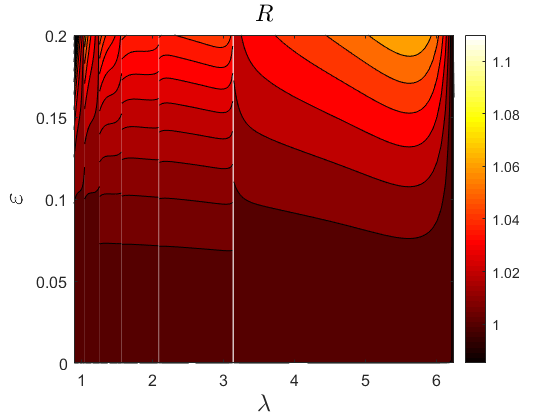
\includegraphics[width=7.6cm]{sections/6_scattering_and_reflectivity/Reflectivity Map TE Base Case.png} }}
    \subfloat[\centering Energy Defect]
    {{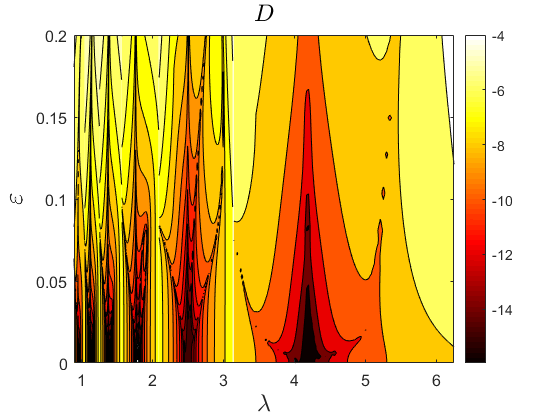
\includegraphics[width=7.6cm]{sections/6_scattering_and_reflectivity/Energy Defect TE Base Case.png} }}
    \vspace{2mm}
    \caption{The Reflectivity Map, $R(\varepsilon,\delta)$, and Energy Defect $D$
    computed with Taylor summation. We set $N=M=15$ 
    with a granularity of $N_{\varepsilon}=N_{\delta}=100$ per invocation. The grating surface was $(6.31)$ and physical parameters were $(6.32)$.}
    \label{Fig:RM:Dielectric}
\end{figure}
\vspace{-18mm}
We then changed to non--normal incidence ($\alpha \neq 0$) and increased the granularity to $N_{\varepsilon}=N_{\delta}=1000$ per invocation. We once again studied
\be
f(x) = \cos(x),
\quad
\varepsilon_{\text{max}} = 0.2,
\quad
a=1,
\quad
b=-1,
\ee
with the parameters
\be
\alpha = 10^{-4},
\quad
\sigma=0.99,
\quad
n^u = 1,
\quad
n^w = 1.1,
\quad 
N_x = N_z = 32,
\quad
N=M=15.
\ee
In Figure $30(\text{a})$ we plot all six of these subsets of the 
Reflectivity Map on one set of coordinate axes, and in 
Figure $30(\text{b})$ we plot the Energy Defect, to verify the accuracy of our expansions.
\vspace{-18mm}
\begin{figure}[H]
    \centering
    \subfloat[\centering Reflectivity Map]
    {{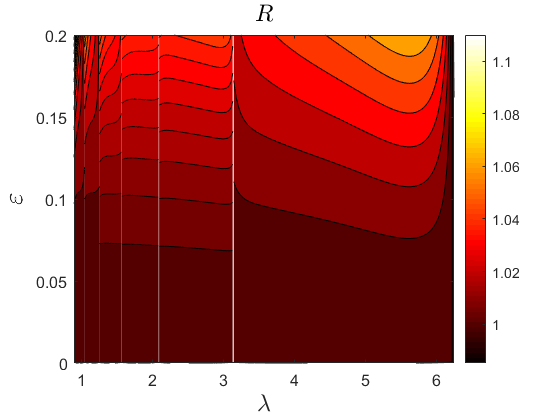
\includegraphics[width=7.6cm]{sections/6_scattering_and_reflectivity/Reflectivity Map TE Base Case With Alpha.png} }}
    \subfloat[\centering Energy Defect]
    {{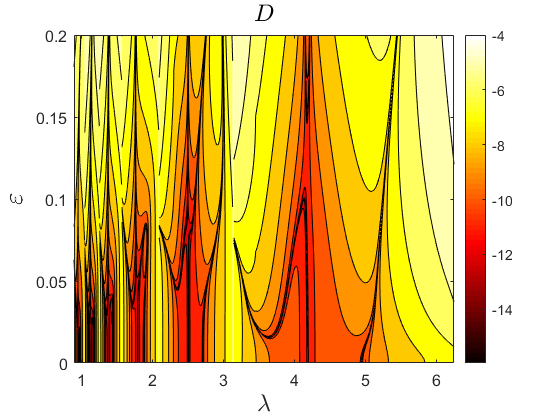
\includegraphics[width=7.6cm]{sections/6_scattering_and_reflectivity/Energy Defect TE Base Case With Alpha.png} }}
    \vspace{3mm}
    \caption{The Reflectivity Map, $R(\varepsilon,\delta)$, and Energy Defect $D$
    computed with Taylor summation. We set $N=M=15$ 
    with a granularity of $N_{\varepsilon}=N_{\delta}=1000$ per invocation. The grating surface was $(6.33)$ and physical parameters were $(6.34)$.}
    \label{Fig:RM:Dielectric}
\end{figure}

\vspace{-17mm}
Next, we considered normal incidence ($\alpha = 0$) and changed the lower index of refraction $n^w$ to match representative values
of copper (Cu) and cobalt (Co) as reported by Johnson \& Christy 
\cite{JohnsonChristy72,johnson1974optical}, in particular
\bes
n_{\text{Cu}} = 0.94 + 1.337i,
\quad
n_{\text{Co}} = 2.1396 + 3.9840i.
\ees
Using the same frequency and wavelength ranges, we studied
\be
f(x) = \sin(5x),
\quad
\varepsilon_{\text{max}} = 0.2,
\quad 
a=2/\pi, 
\quad 
b = -2/\pi,
\ee
with the parameters
\be
\alpha = 0,
\quad
\sigma=0.99,
\quad
n^u = 1,
\quad
N_x = N_z = 32,
\quad
N=M=15.
\ee
In Figure $31(\text{a})$ we plot six different subsets of the Reflectivity
Map where the lower index of refraction is selected to model the optical constant
of copper. In Figure $31(\text{b})$ we plot six different subsets of 
the Reflectivity Map where the lower index of refraction is changed to the optical
constant for cobalt.
%
% Figure: Reflectivity Map for Metals
%
\vspace{-18mm}
\begin{figure}[H]
    \centering
    \subfloat[\centering Reflectivity Map for Copper]
    {{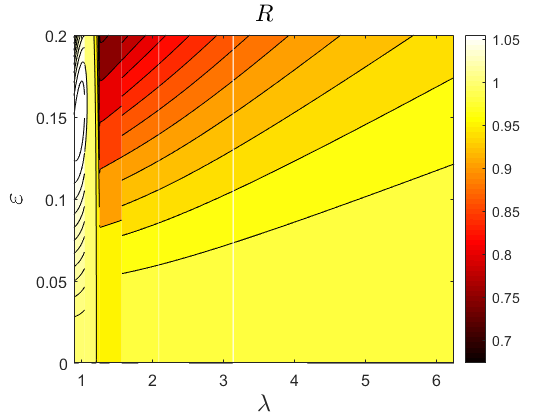
\includegraphics[width=7.6cm]{sections/6_scattering_and_reflectivity/Reflectivity Map for Copper.png} }}
    \subfloat[\centering Reflectivity Map for Cobalt]
    {{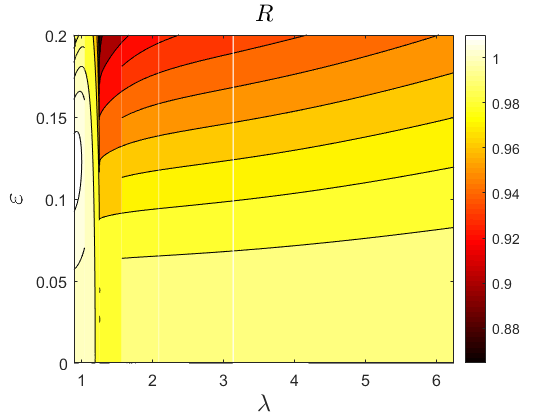
\includegraphics[width=7.6cm]{sections/6_scattering_and_reflectivity/Reflectivity Map for Cobalt.png} }}
    \vspace{.15mm}
    \caption{The Reflectivity Map, $R(\varepsilon,\delta)$, for copper (left)
    and cobalt (right) with
    Pad\'e summation. We set $N=M=15$ with a granularity
    of $N_{\varepsilon}=N_{\delta}=100$ per invocation. The grating surface was $(6.35)$ and physical parameters were $(6.36)$ with $n^w = n_{\text{Cu}}$ (left)
    and $n^w = n_{\text{Co}}$ (right).}
    \label{Fig:RM:Metal}
\end{figure}
\vspace{-20mm}

We then analyzed non--physical values of the dielectric constants. We simulated $R$ with the first frequency/wavelength range in $(6.3)$ and selected
\be
f(x) = \cos(x),
\quad
\varepsilon_{\text{max}} = 0.2,
\quad 
a=\pi/2, 
\quad 
b = -\pi/2,
\ee
with a purely imaginary index of refraction in the lower layer
\be
\alpha = 0.001,
\quad
\sigma=0.99,
\quad
n^u = 5,
\quad
n^w = 20i,
\quad
N_x = N_z = 32,
\quad
N=M=15.
\ee
%\vspace{-23mm}
In Figure $32$ we plot the
Reflectivity Map and Energy Defect on a single coordinate axis to demonstrate the accuracy of our
scheme with a non--physical dielectric constant.

%
% Figure: Reflectivity Map for Non-Physical Dielectric
%
\vspace{-23mm}
\begin{figure}[H]
    \centering
    \subfloat[\centering Reflectivity Map]
    {{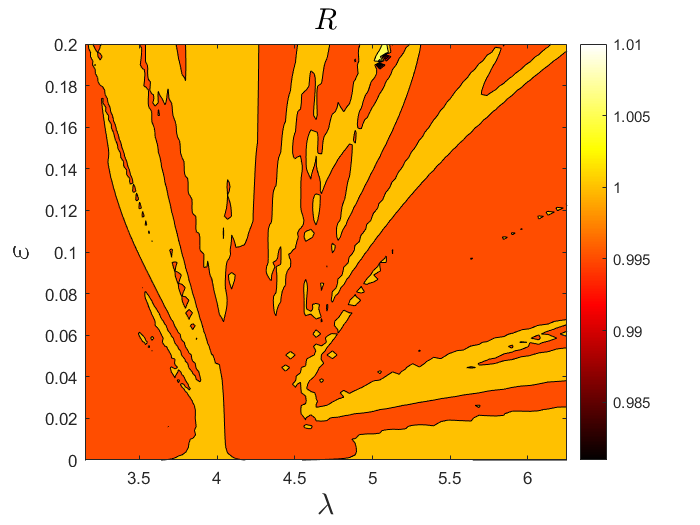
\includegraphics[width=7.6cm]{sections/6_scattering_and_reflectivity/Reflectivity Map TE NonPhysical.png} }}
    \subfloat[\centering Energy Defect]
    {{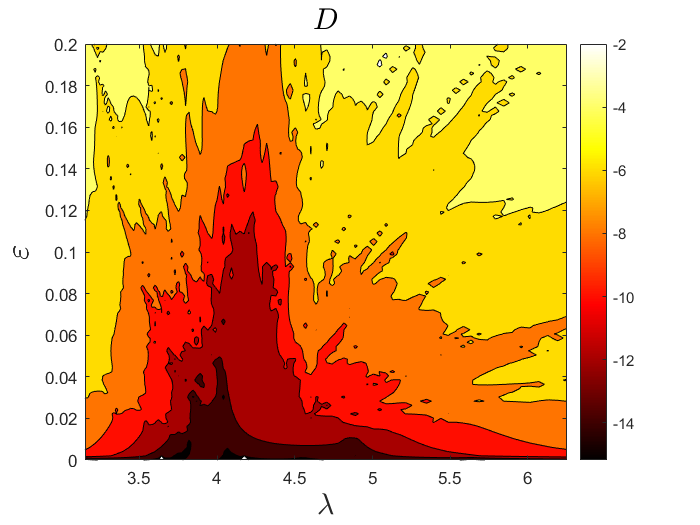
\includegraphics[width=7.6cm]{sections/6_scattering_and_reflectivity/Energy Defect TE NonPhysical.png} }}
    \vspace{.15mm}
    \caption{The Reflectivity Map, $R(\varepsilon,\delta)$, and Energy Defect $D$
    computed with Pad\'e summation. We set $N=M=15$ 
    with a granularity of $N_{\varepsilon}=N_{\delta}=100$ per invocation. The grating surface was $(6.37)$ and physical parameters were $(6.38)$.}
    \label{Fig:RM:Single Case 1}
\end{figure}
\vspace{-17mm}
\hspace{-6mm}Lastly, we selected
\be
f(x) = \sin(x),
\quad
\varepsilon_{\text{max}} = 0.2,
\quad
a=2/\pi, 
\quad 
b = -2/\pi,
\ee
and
\be
f(x) = \cos(x),
\quad
\varepsilon_{\text{max}} = 0.2,
\quad
a=2/\pi, 
\quad 
b = -2/\pi,
\ee
with the parameters
\be
\alpha = 0.1,
\quad
\sigma=0.99,
\quad
n^u = 10,
\quad
n^w = 25i,
\quad
N_x = N_z = 32,
\quad
N=M=15.
\ee
In Figures $33(\text{a})$ and  $33(\text{b})$ we plot the Reflectivity Map and Energy Defect for the sine profile on a single coordinate axis and compare this to an equivalent simulation for the cosine profile in Figures $33(\text{c})$ and  $33(\text{d})$.

\vspace{-21mm}
\begin{figure}[H]
    \centering
    \subfloat[\centering Reflectivity Map]
    {{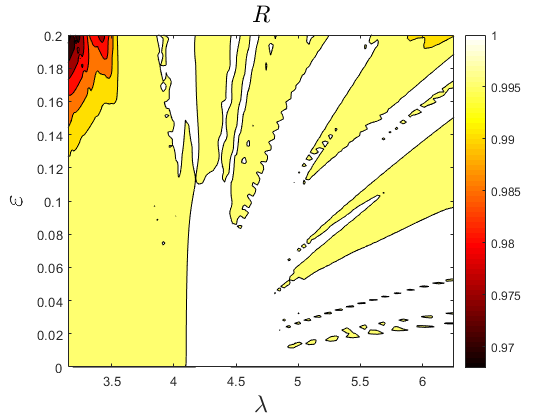
\includegraphics[width=7.6cm]{sections/6_scattering_and_reflectivity/Reflectivity Map TE NonPhysical 2.png} }}
    \subfloat[\centering Energy Defect]
    {{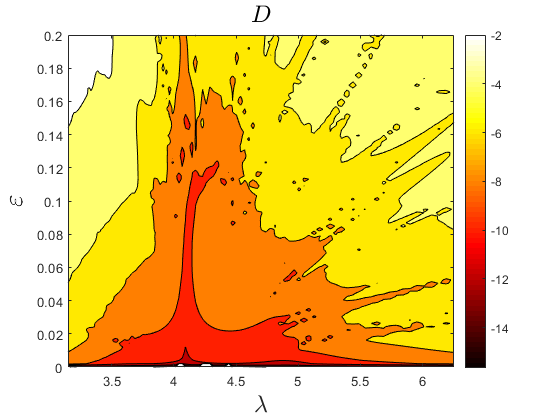
\includegraphics[width=7.6cm]{sections/6_scattering_and_reflectivity/Energy Defect TE NonPhysical 2.png} }}
    \\
    \subfloat[\centering Reflectivity Map]
    {{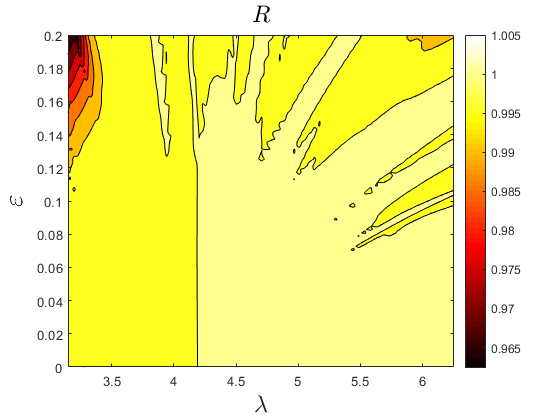
\includegraphics[width=7.6cm]{sections/6_scattering_and_reflectivity/Reflectivity Map TE NonPhysical 3.png} }}
    \subfloat[\centering Energy Defect]
    {{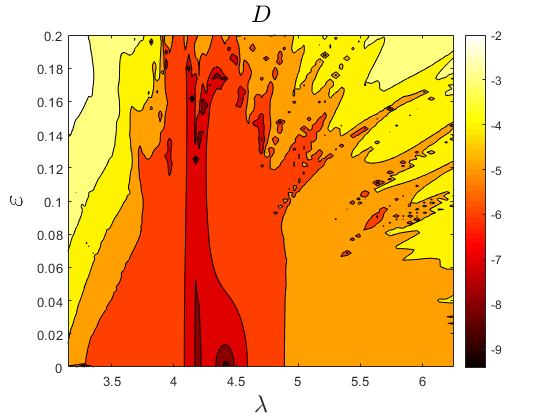
\includegraphics[width=7.6cm]{sections/6_scattering_and_reflectivity/Energy Defect TE NonPhysical 3.png} }}
    \vspace{3mm}
    \caption{The Reflectivity Map, $R(\varepsilon,\delta)$, and Energy Defect $D$
    computed with Pad\'e summation. We set $N=M=15$ 
    with a granularity of $N_{\varepsilon}=N_{\delta}=100$ per invocation. (Top) The grating surface was $(6.39)$ and physical parameters were $(6.41)$. (Bottom) The grating surface was $(6.40)$ and physical parameters were $(6.41)$.}
    \label{Fig:RM:Single Case 1}
\end{figure}